\chapter{$Z\to\tauh\taul$ tag and probe study}\label{chap1}
This chapter describes the analysis methodology of using $Z\to\tau\tau$ events to measure Monte Carlo correction factors for tau identification algorithms on the high-$p_T$ region.

As we saw in the previous section different working points are defined for RNN score relative to the efficiency of selecting true $\tauh$ candidates. When the efficiency of the working points is measured in data and simulation, a correction factor is derived and then applied to the simulation in order for the signal efficiency to agree between data and simulation REF TAU ID PERFORMANCE. Because of the top quark mass, $t\bar{t}$ events are used as a source of high momentum taus for measuring correction factors on the high-$p_T$ bins. But as we already saw in section \ref{chap2sec2}, LU may not hold on W decays. For that reason our study is aimed to use $Z\to\tau\tau$ events for deriving simulation correction factors on the high-$p_T$ region.   

\section{Signal events}\label{chap4sec1}
The type of $Z\to\tau\tau$ events we consider as signal are when one the taus decays hadronically and the other leptonically, either into an electron or a muon ($Z\to\tau\tau\to\tau_h +l=\mu,e$). Thus, our final states will include a $\tauh$ candidate and a lepton $l=e,\mu$. The presence of this lepton will be used as our tag. 
Generally, in $Z\to\tau\tau$ events, the taus are produced back to back and their $\pt$ spectrum does not go very high. One way to select events where the taus are boosted on the transverse plain is to look for events where the opening angle in the transverse plane between the taus ($\Delta\phi(\tauh,\taul)$) is more acute. For these events, the missing transverse momentum ($\ptmiss$) is assumed to come from the neutrinos produced in the decays of the tau leptons. Due to the fact that two neutrinos are produced in the leptonic decay mode we expect our events to have a larger $\ptmiss$ component along the $\taul$ direction.

We classify our events in two types of topologies. First, events where the $\ptmiss$ is inside the opening angle between the visible objects, in this kind of events we assume the missing energy is due to a pair of neutrinos flying in the same direction as the visible objects. This is shown in Fig.\ref{Fig7a} . In this case, we solve the following equation to obtain the momentum of the neutrinos:
\begin{equation}
	\vec{p}_{T_{\nu_l}}+\vec{p}_{\nu_h}=\vec{p}_{T_{\text{miss}}},
\end{equation}
given the following set of constraints (\textit{collinear approximation}):
\begin{align}
	\phi(\nu_l)&=\phi(l),
	\\
	\phi(\nu_h)&=\phi(\tauh),
	\\
	\eta(\nu_l)&=\eta(l),
	\\
	\eta(\nu_h)&=\eta(\tauh).
\end{align}
The second case is when the $\ptmiss$ is outside the angle formed by the visible objects, as is shown in Fig.\ref{Fig7b}, in this case the assumption is that only one neutrino is responsible for the majority of the $\ptmiss$, a neutrino flying in the direction of the visible object that is closest to the $\ptmiss$. We use the following equations to obtain the neutrino momentum:
\begin{align}
p_{T_{\nu}}&=\ptmiss \cos(\Delta\phi(\tau_{\text{closer}},\ptmiss)),
\\
\phi(\nu)&=\phi(\tau_{\text{closer}}),
\\
\eta(\nu)&=\eta(\tau_{\text{closer}}),
\end{align} 
\begin{figure}[ht]
	\centering
	\subfloat[]{\label{Fig7a}{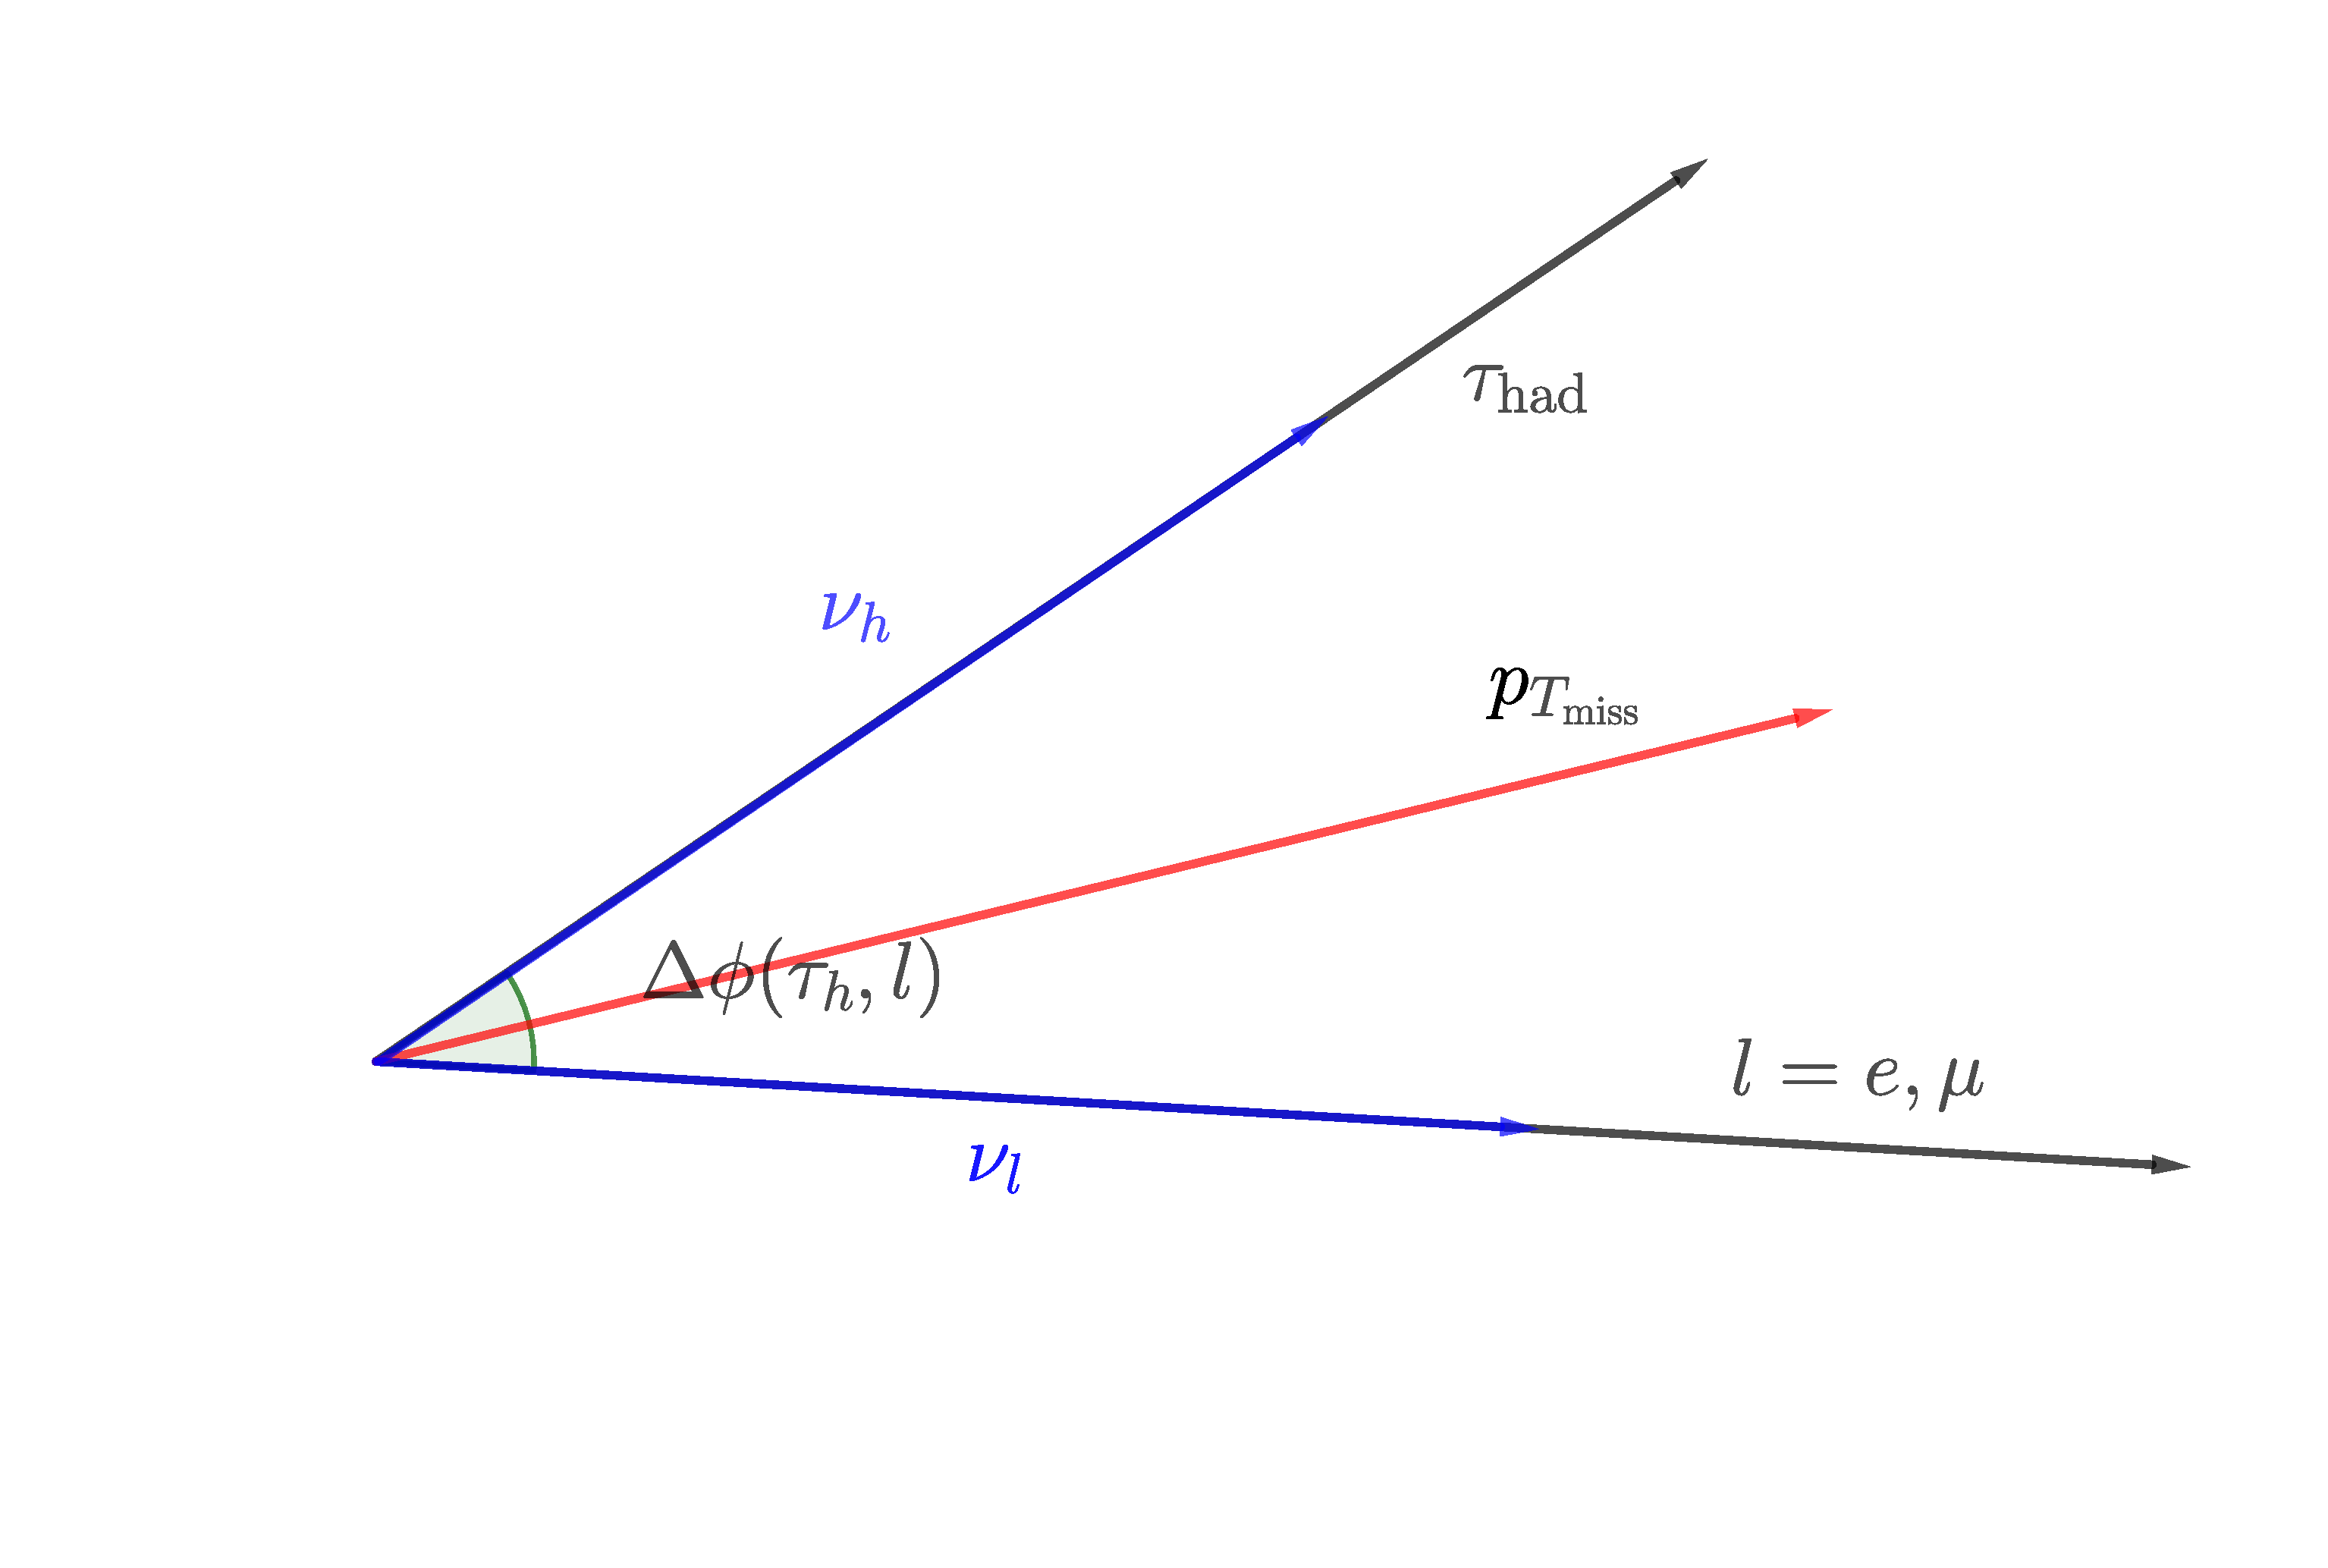
\includegraphics[width=0.45\textwidth]{figures/Fig7a}}}\hfill
	\subfloat[]{\label{Fig7b}{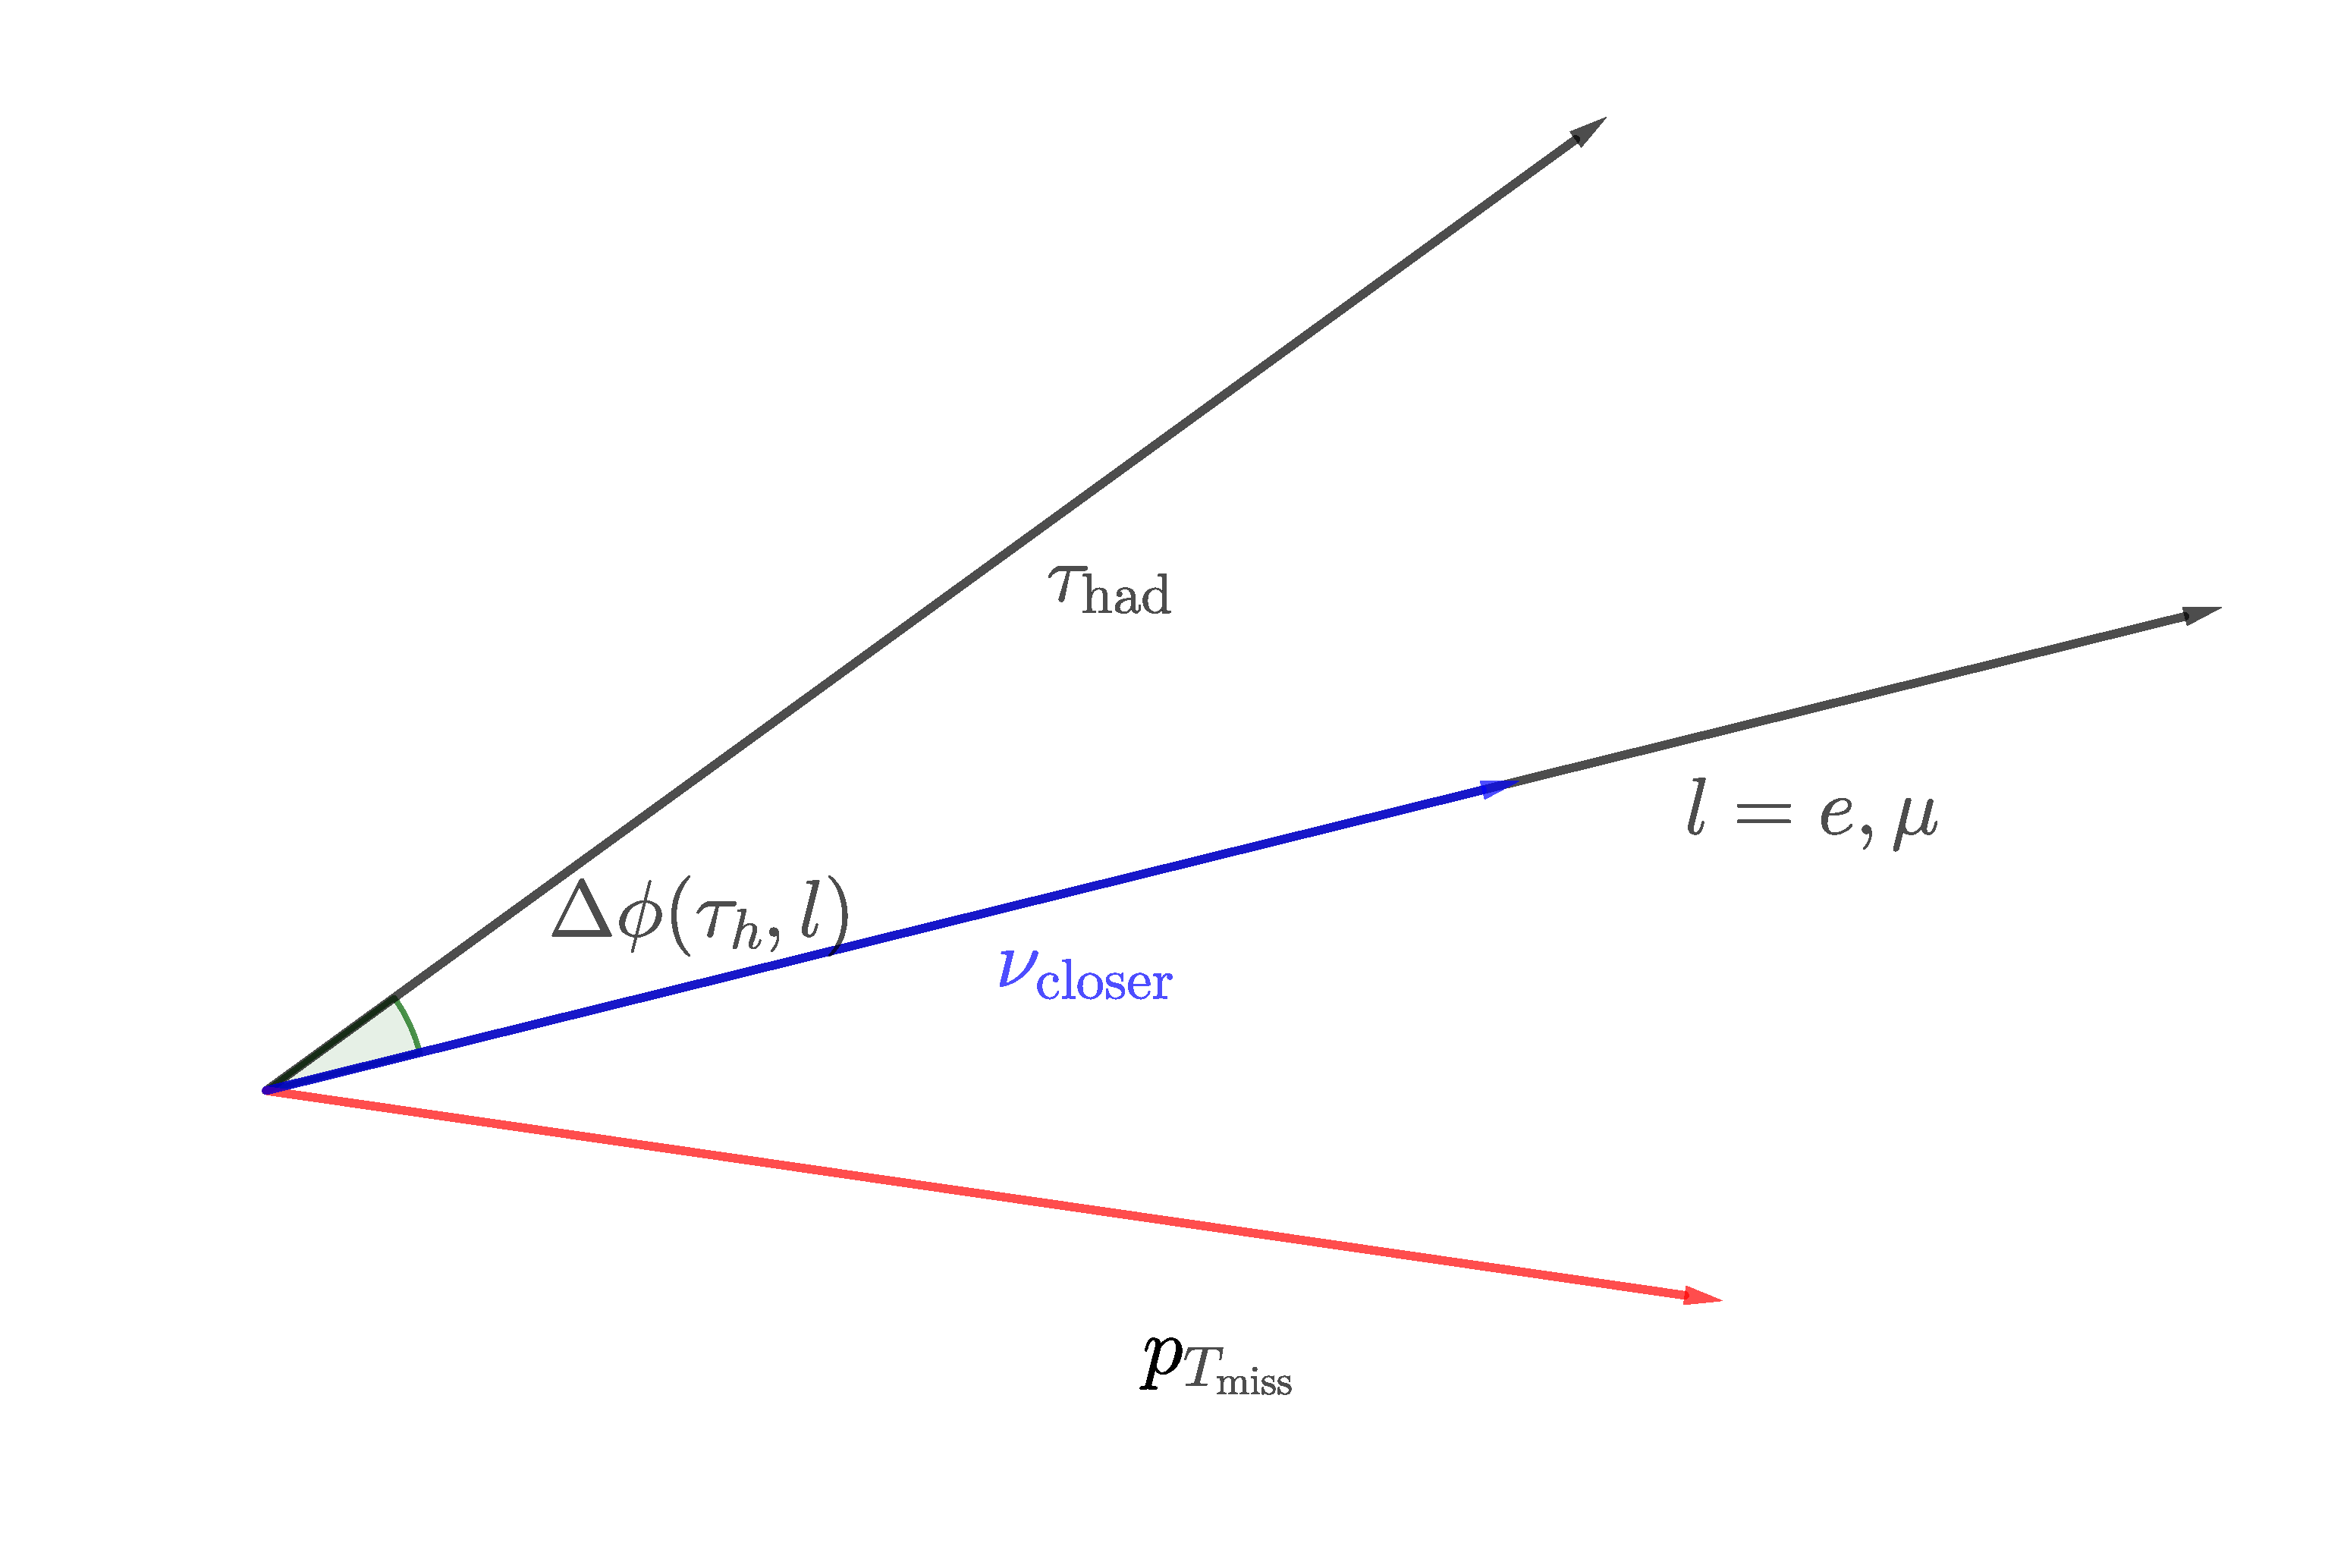
\includegraphics[width=0.45\textwidth]{figures/Fig7b}}}
	\caption{The two different types of topologies that define signal events. On the right, when the missing energy is between the visible objects two neutrinos are assumed to be responsible for all the missing energy. On the left, only one neutrino is assumed to be flying on the direction of the visible object closest to the missing energy.}
	\label{Fig7}
\end{figure}
where $\tau_{closer}$ stands for the visible object closest to the direction of the missing energy.

We define a variable called $\Omega$ in order to classify our events in the different topologies already described. First we define:
\begin{equation}
	\omega=\frac{\Delta\phi(\tau_{\text{close}},\ptmiss)}{\Delta\phi(\tauh,\taul)},
\end{equation}
then,
\begin{itemize}
	\item when $\ptmiss$ is inside the opening angle between the visible objects but closer to $\tauh$:
	\begin{equation}
		\Omega=\omega,
	\end{equation}
	\item when $\ptmiss$ is still inside, but closer to $\taul$:
	\begin{equation}
		\Omega=1-\omega.
	\end{equation}
	\item If $\ptmiss$ is outside and closer to $\tauh$:
	\begin{equation}
		\Omega=-\omega,
	\end{equation}
	\item and finally, if $\ptmiss$ is outside and closer to $\taul$:
	\begin{equation}
		\Omega=\omega+1.
	\end{equation}
\end{itemize}
Thus, $\Omega$ is a continuous variable that give us information on the topology of the event. When $\ptmiss$ is inside the visible system it has values in the interval [0,1]. Exactly 0 when $\ptmiss$ is in the $\tauh$ direction and 1 when is on the $\taul$ direction. $\Omega$ has negative values when $\ptmiss$ is outside and closer to the $\tauh$ candidate and has positive and values greater than 1 when is outside and closer to the $\taul$. A diagram describing the $\Omega$ values is shown in Fig.\ref{Fig8}.
\begin{figure}[h]
	\centering
	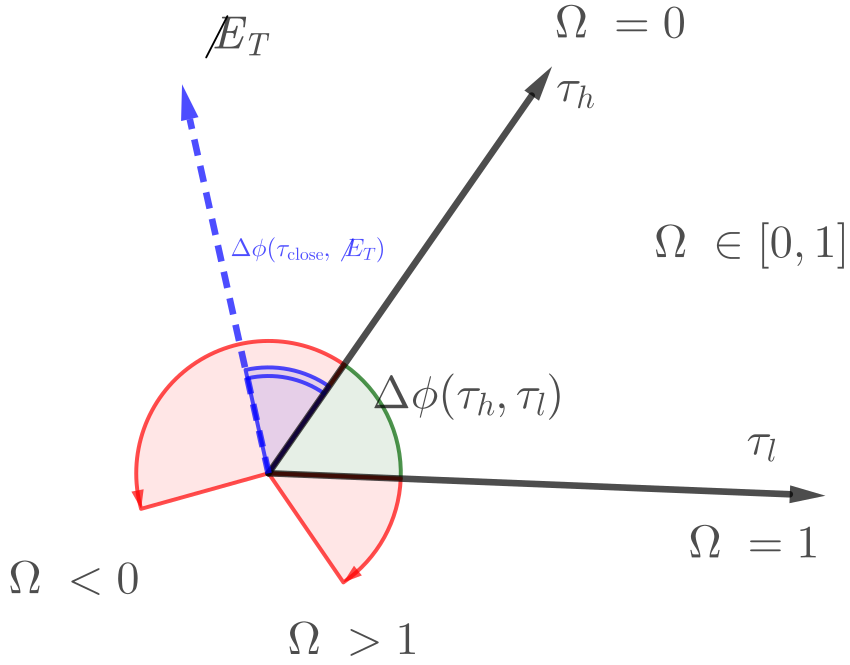
\includegraphics[width=0.5\textwidth]{figures/Fig8}
	\caption{Graphical representation of the different values of $\Omega$ depending on the region where the $\ptmiss$ is located in the event.}
	\label{Fig8}
\end{figure}
As we will see later the event classification into this two different type of topologies will allow us to reconstruct and exploit kinematical variables as the invariant mass of the di-tau system, the Z boson transverse momentum ($Z_{p_T}$) and the angular distribution of the objects in the event.
\section{Monte Carlo and Data Samples}
The data used for this study has been recorded during the Run-II of the LHC. This corresponds to the 2015-2018 data taking period, the total integrated luminosity corresponds to 139.2 $\text{fb}^{-1}$ of proton-proton collisions at a centre-of-mass energy of $\sqrt{s}=13$ TeV.

Monte Carlo (MC) samples are used for signal and background simulation. For $Z\to\tau\tau$ events two MC samples are used, Powheg+Pythia8 and Sherpa. For the rest of the samples Powheg+Pythia8 is used. Table \ref{Table3} shows the MC generators used for each process.

\begin{table}[]
	\centering
	\begin{tabular}{cc}
		\hline
		\multicolumn{1}{|c|}{Process}  & \multicolumn{1}{c|}{Event Generator} \\ \hline
		$Z\to\tau\tau$                 & Powheg+Pythia8 and Sherpa            \\
		$Z\to ee$                      & Powheg+Pythia8                       \\
		$Z\to\mu\mu$                   & Powheg+Pythia8                       \\
		$W\to l\nu_l$				   & Powheg+Pythia8                       \\
		$t\bar{t}$                     & Powheg+Pythia8                       \\
		Single $t$                     & Powheg+Pythia8                       \\
		Diboson                        & Powheg+Pythia8                       \\ \hline
	\end{tabular}
	\caption{List of MC event generators used.}
	\label{Table3}
\end{table}
\section{Event Selection}\label{chap4sec3}
The basic selection for our $Z\to\tauh\taul$ includes events with exactly one $\tauh$ candidate and one lepton, a muon or an electron. The $\tauh$ and lepton pair need to have opposite charge. As we said, the presence of the lepton will be used as our tag, thus, a lepton trigger is required to be fired with an online requirement on the $p_{T}(\mu)\geq 20$ ($p_{T}(e)\geq 24$) GeV for 2015 data taking period. For 2016-2018 the requirement is $p_{T}(\mu,e)\geq 26$ GeV. The muons are required to pass a \textit{medium} ID requirement and the electron has to pass a \textit{tight} ID filter. Additionally, both muons and electrons have to pass an offline $p_T$ requirement to be greater than 27 GeV. Finally, the opening angle between the two visible objects $\Delta\phi(\tauh,l)\leq 2\pi/3$.

Events containing b jets are vetoed in order to reject $t\bar{t}$ events. Also an isolation criteria is required to be passed by the leptons: for the muon (electron), the scalar sum of the $p_T$ of the tracks within a cone of $\Delta R=0.3 (0.2)$ of the muon (electron) must be less than 0.06 times the muon (electron) $p_T$. Aditionally for the electron, the sum of the calorimeter cluster energy in a cone of size $\Delta R=0.2$ must be 0.06 times the electron $p_T$.  Then, as we said in section \ref{chap4sec1}, we expect signal events to peak around $\Omega=1$, thus we select events where $\Omega\in (0,1.4)$. Fig.\ref{Fig9} shows the $\Omega$ distribution for $Z\to\tauh\mu$ final state.
\begin{figure}[h]
	\centering
	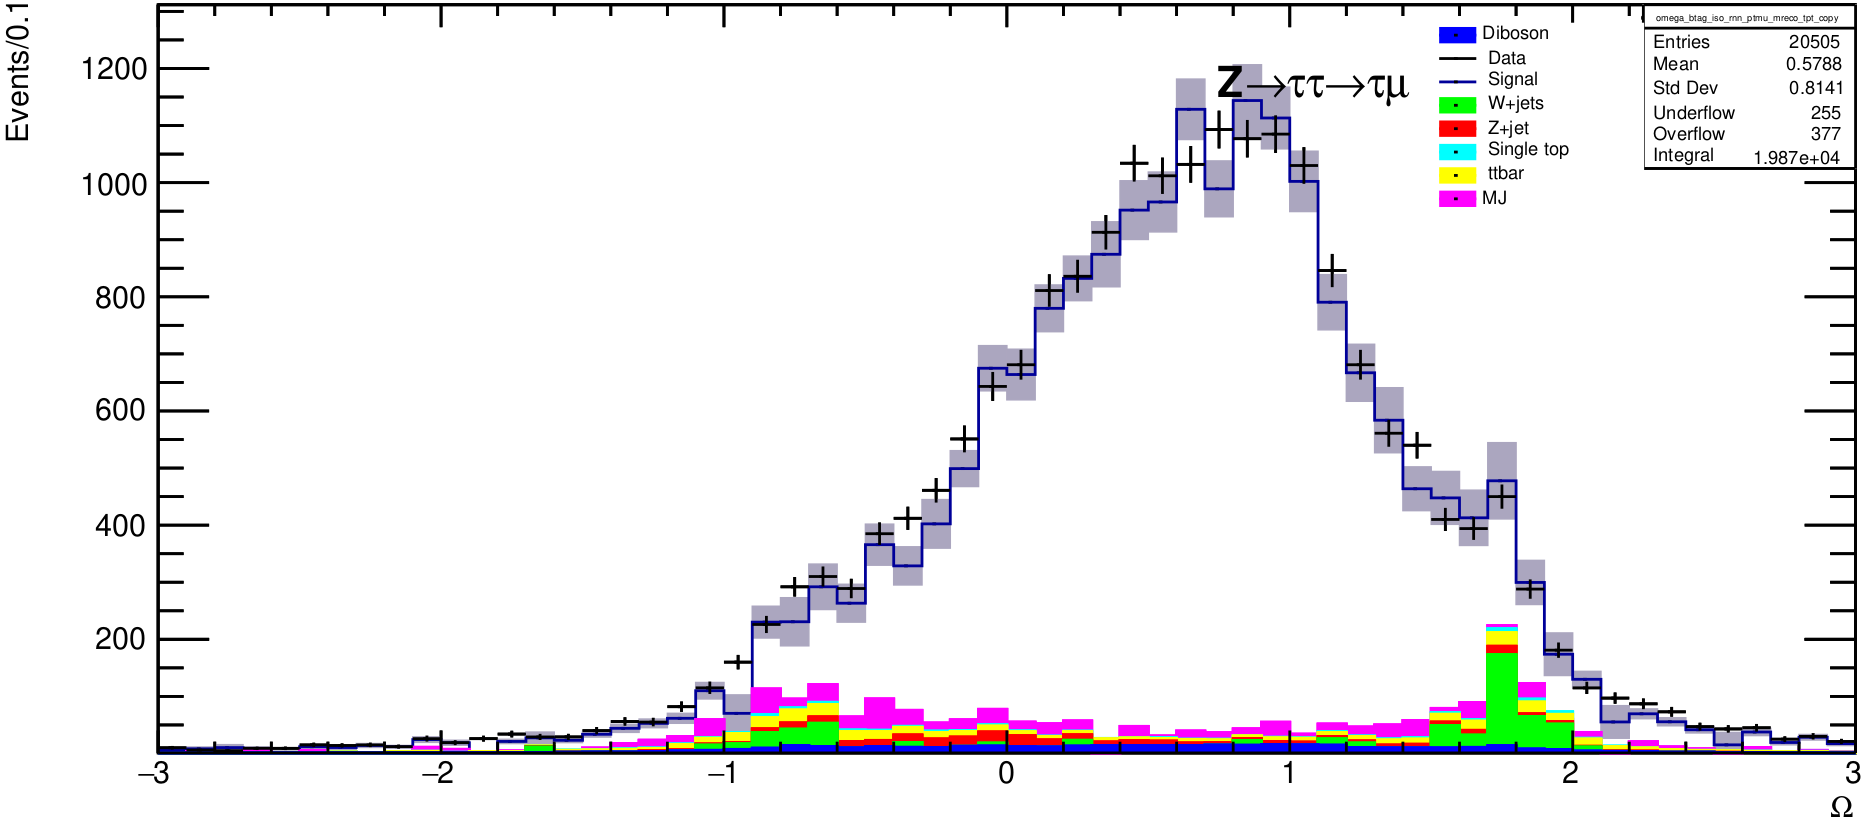
\includegraphics[width=0.7\textwidth]{figures/Fig9}
	\caption{Distribution of $\Omega$ for $Z\to\tauh\mu$ final state. }
	\label{Fig9}
\end{figure}
Adittionally, a cut on the reconstructed invariant mass ($\mreco$) of the event is made, the cut aims to pick events where the invariant mass is around the Z boson mass ($70\leq\mreco\leq 110$ GeV). The invariant mass of the final states is calculated depending on the event topology. For events where $\Omega\in [0,1]$ (\textit{in between events}),  $\mreco^{2}=(q_l+q_{\tauh}+q_{\nu_l}+q_{\nu_{\tauh}})^2$ and when the $\ptmiss$ is outside (\textit{outside events}), $(\mreco-5)^{2}=(q_l+q_{\tauh}+q_\nu)^2$. In the latter case we manually add 5 GeV to maintain our cuts consistent, since in this region the Z mass is underestimated. Fig. shows the distribution of $\mreco$ for the in between and outside $Z\to\tauh\mu$ events. 
\begin{figure}[ht]
	\centering
	\subfloat[]{\label{Fig10a}{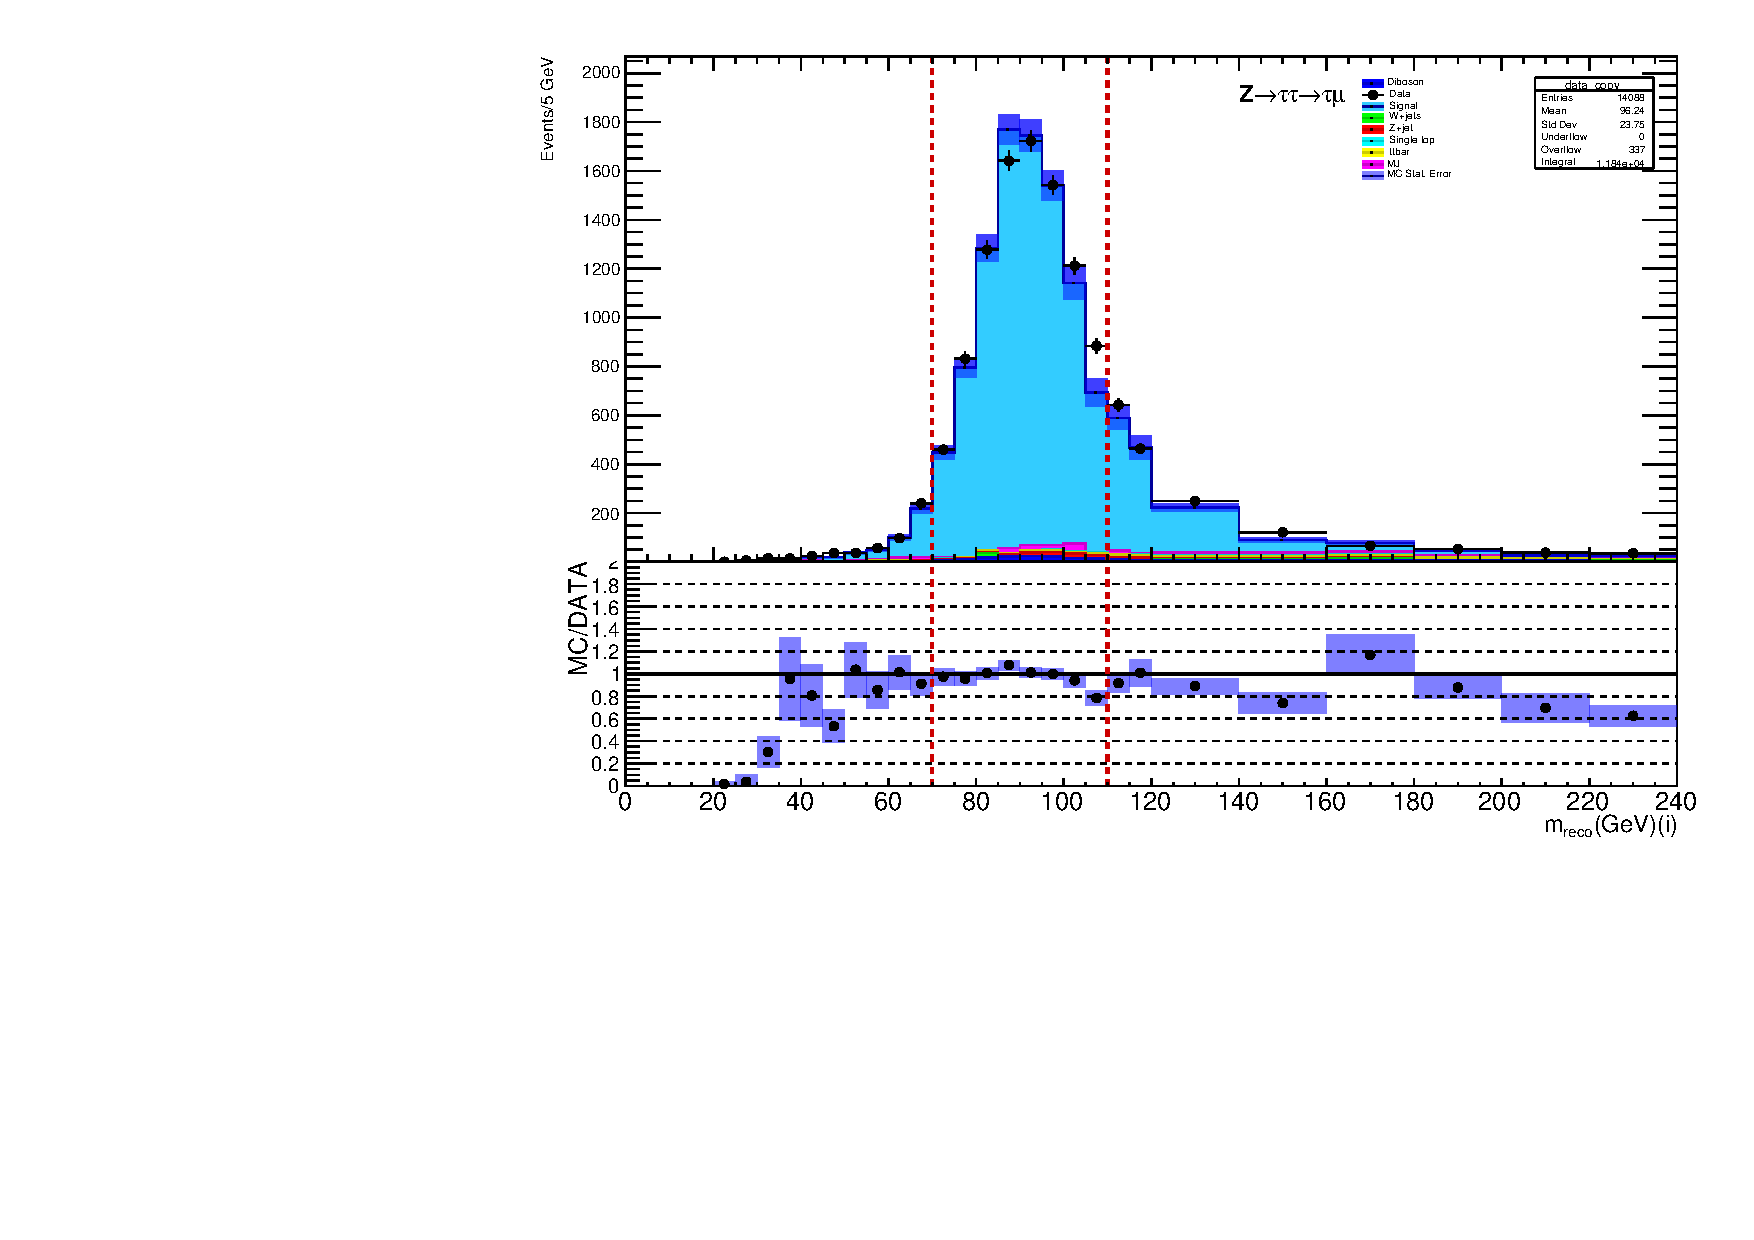
\includegraphics[width=0.50\textwidth]{figures/Fig10a}}}\hfill
	\subfloat[]{\label{Fig10b}{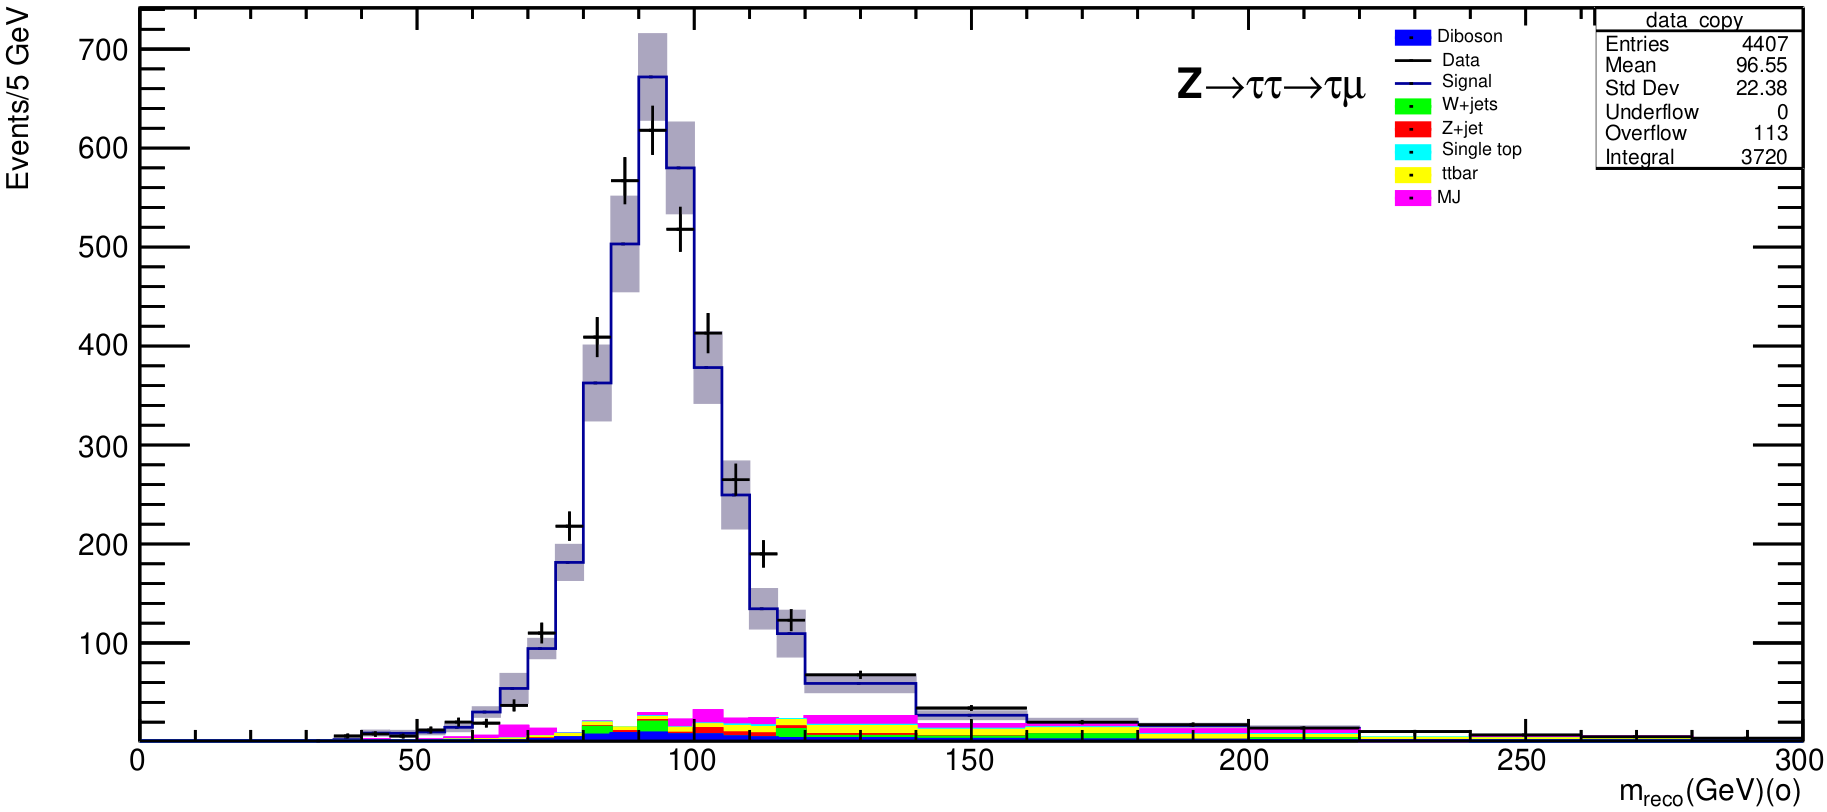
\includegraphics[width=0.50\textwidth]{figures/Fig10b}}}
	\caption{$\mreco$ distribution for the in between region (a) and the outside region (b).}
	\label{Fig10}
\end{figure}

In addition, for the $Z\to\tauh e$ final state, we add two cuts aimed to reject events where the $\tauh$ candidate is faked by an electron. First to reject $Z\to ee$ events, a requirement on the invariant mass of the electron and $\tauh$ candidate is made, $m(e,\tauh)<80$ GeV. Then, we also make use of an ID algorithm to discriminate electrons from real $\tauh$. In our case, eBDTScore$\geq 0.06$. The distributions for this variables are shown in Fig.\ref{Fig11}.
\begin{figure}[ht]
	\centering
	\subfloat[]{\label{Fig11a}{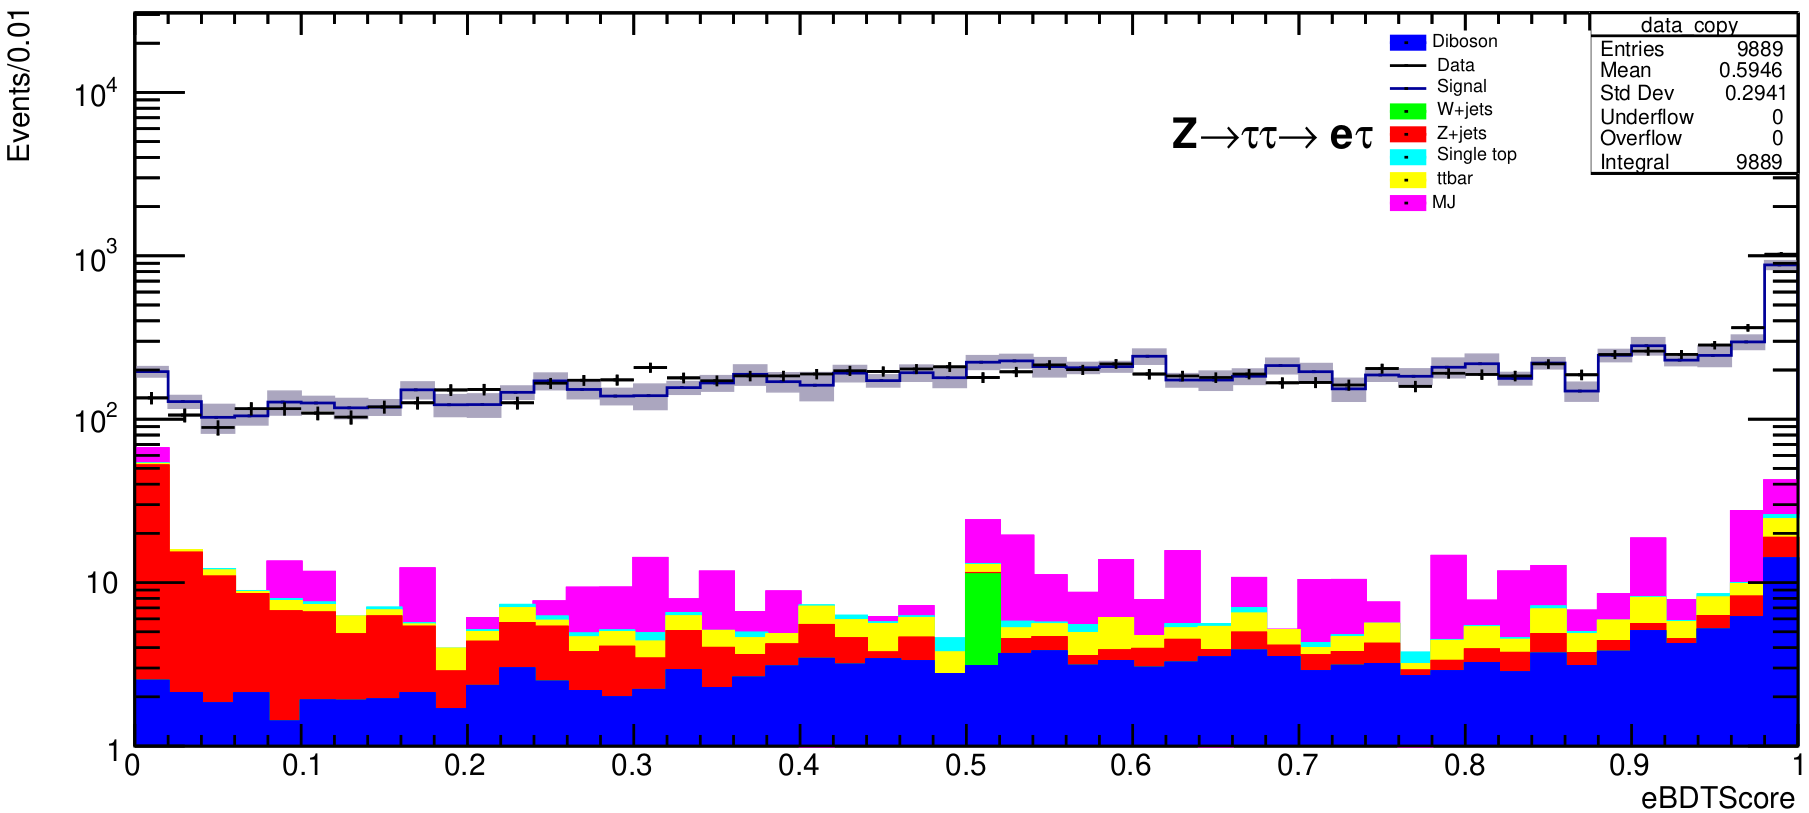
\includegraphics[width=0.50\textwidth]{figures/Fig11a}}}\hfill
	\subfloat[]{\label{Fig11b}{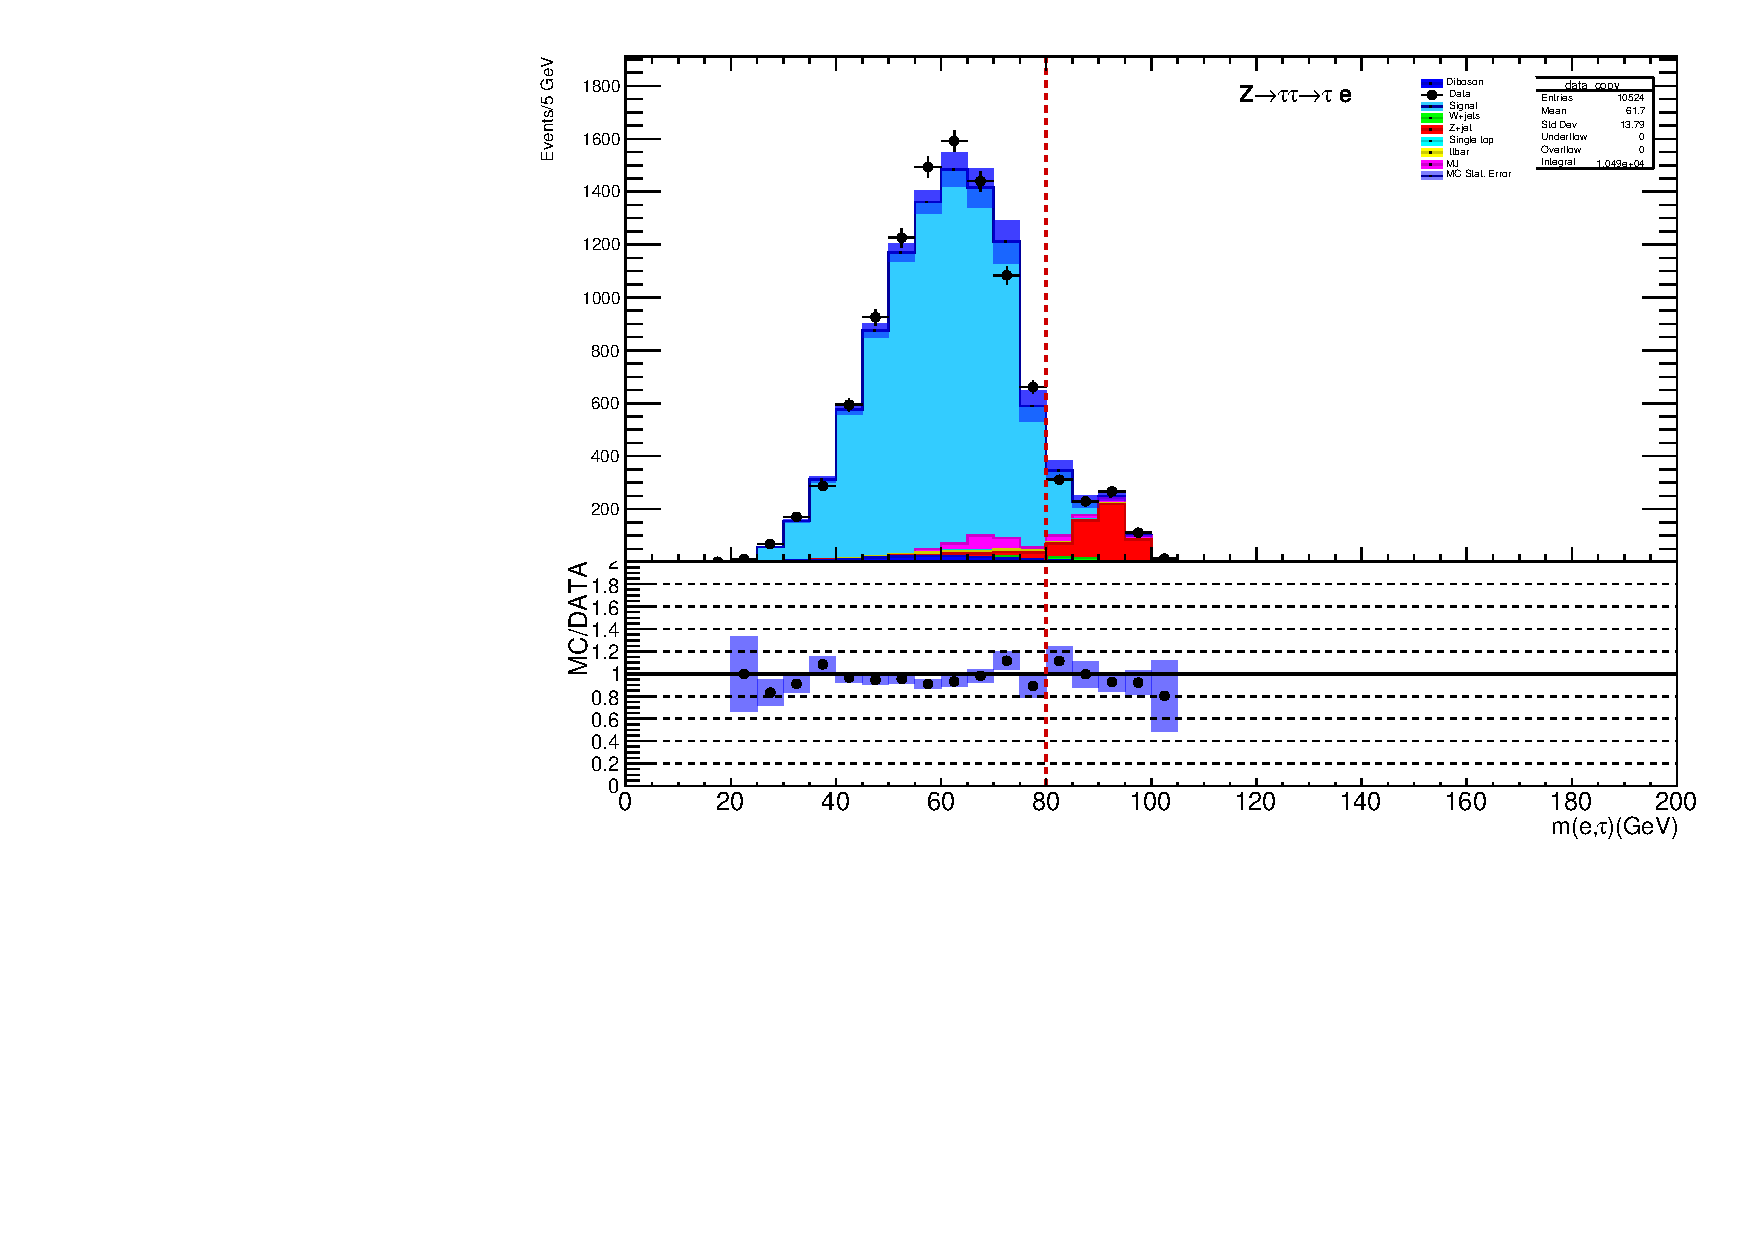
\includegraphics[width=0.50\textwidth]{figures/Fig11b}}}
	\caption{Distribution of the variables used for rejecting $\tauh$ fakes coming from electrons. On the right $m(e,\tauh)$ distribution (a) and on the left the eBDTScore distribution (b).}
	\label{Fig11}
\end{figure}
Finally, in order to measure the tau ID scale factors on the high-$p_T$ region we select events where $p_T(\tauh)\geq 45$ GeV. The $p_T$ distributions for $\tauh$ candidates are shown in Fig.\ref{Fig12} for the in between and outside regions.
\begin{figure}[ht]
	\centering
	\subfloat[]{\label{Fig12a}{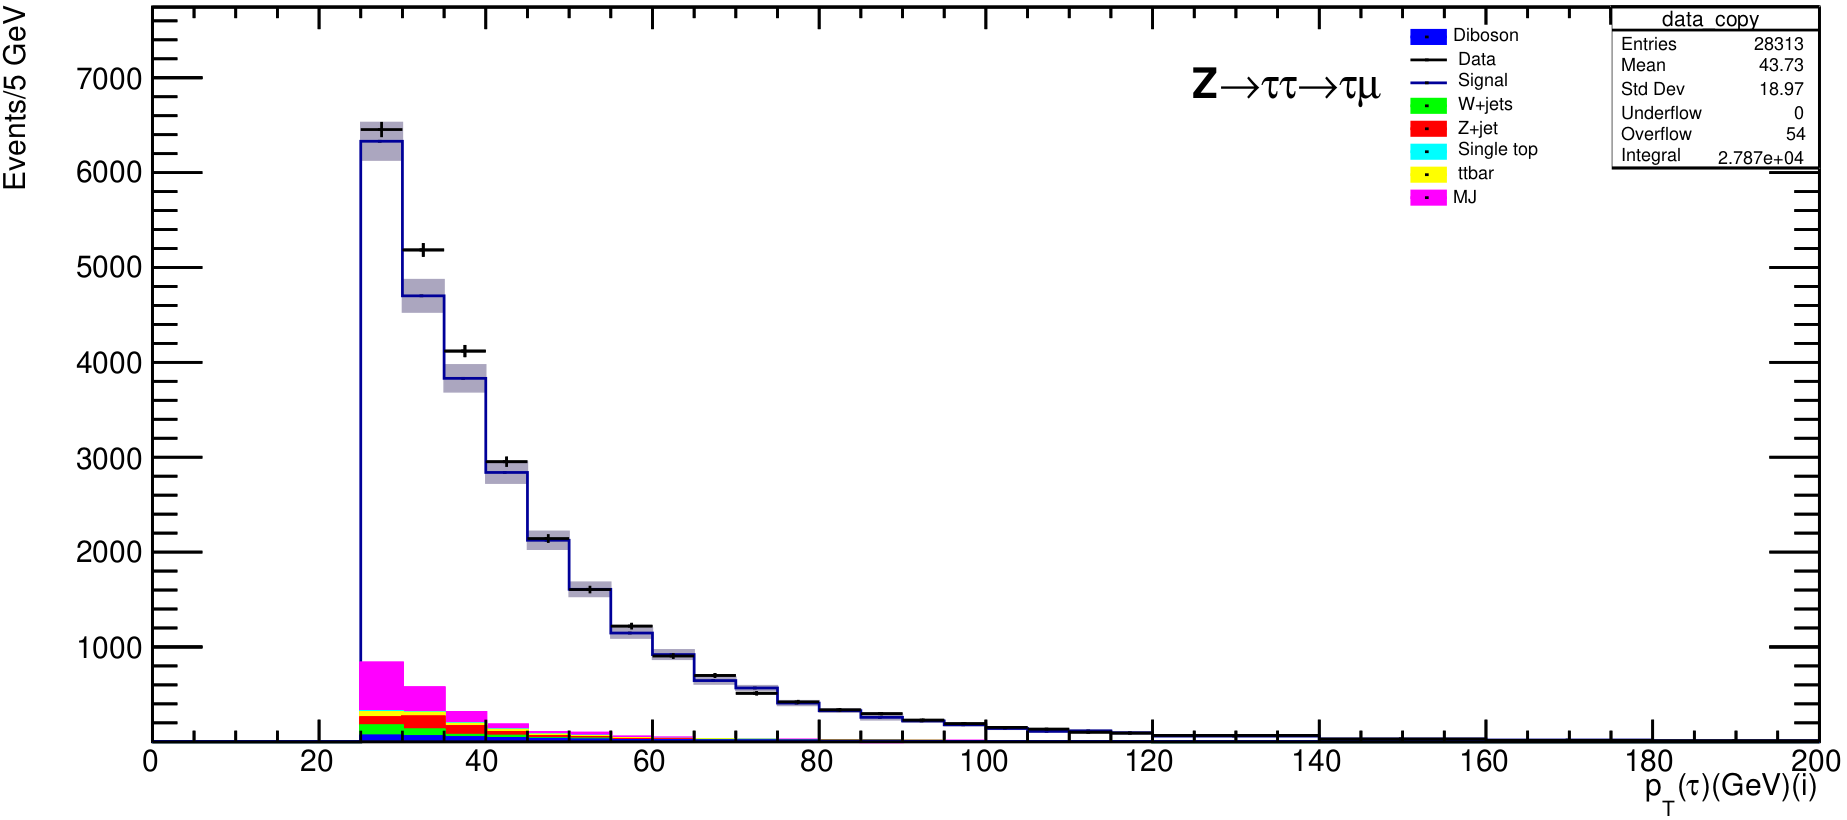
\includegraphics[width=0.50\textwidth]{figures/Fig12a}}}\hfill
	\subfloat[]{\label{Fig12b}{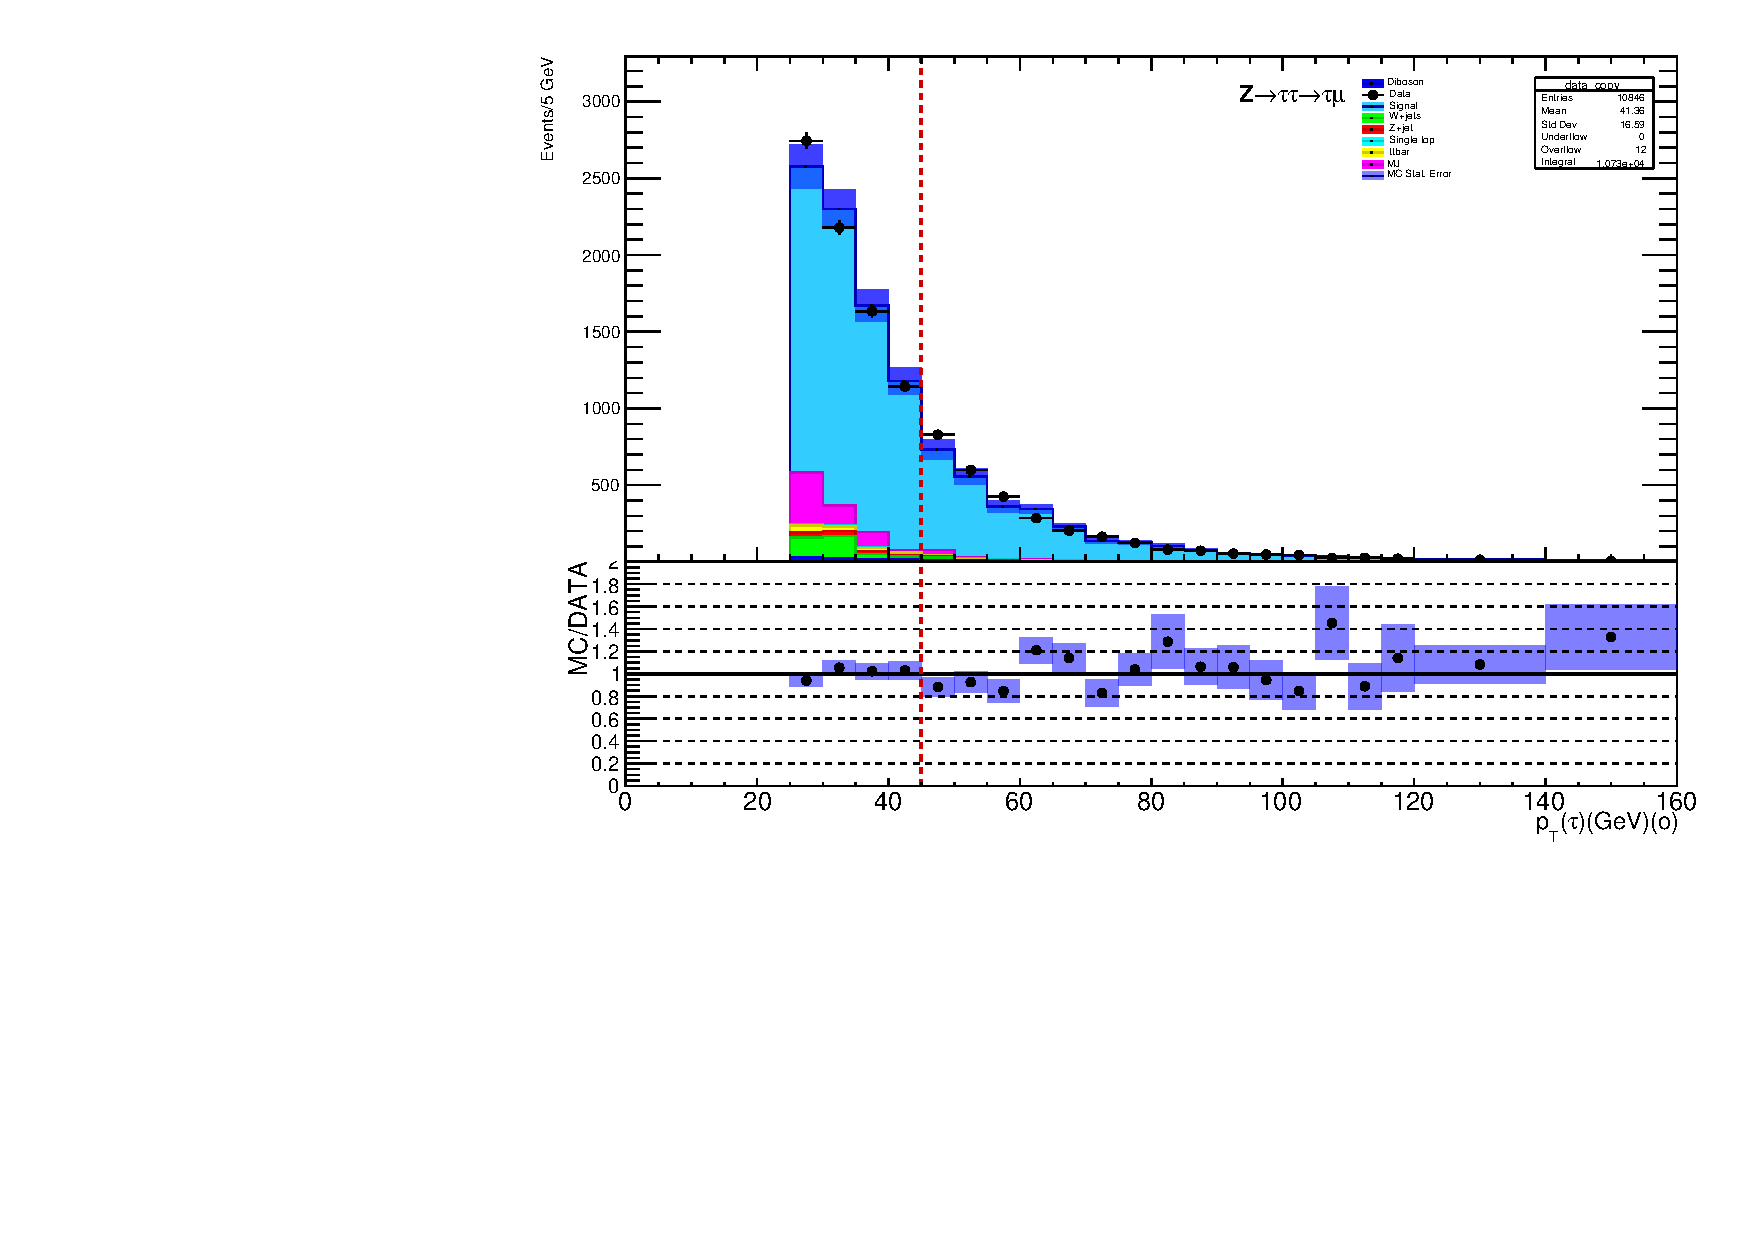
\includegraphics[width=0.50\textwidth]{figures/Fig12b}}}
	\caption{$p_T(\tauh)$ distribution for the in between (a) and outside (b) regions.}
	\label{Fig12}
\end{figure} 
\section{Multi Jet Background Estimation}
As we said previously, $\tauh$ candidates are seeded by jets, thus, QCD events represent a source of background. Nonetheless, we do not have MC simulations for this processes as with the EW interactions shown in Table \ref{Table3}. For this reason, we use a \textit{data driven method} to estimate multi jet (MJ) background. For that purpose, we choose a variable that in principle we suppose is uncorrelated with the shape of the MJ background. For our study, this variable is the relative sign between the charges of the $\tauh$ and the lepton. Thus, this defines two regions: the same sign (SS) region where $q(\tauh)=q(l)$ and the opposite sign region where $q(\tauh)=-q(l)$. Our estimate of MJ background for the SS region is obtained subtracting signal and electroweak backgrounds (EWBG) simulated contributions, basically:
\begin{equation}
\text{MJBG}_{\text{SS}}=\text{Data}_{\text{SS}}-\text{Signal}_{\text{SS}}-\text{EWBG}_{\text{SS}},
\end{equation}
 To study the residual charge correlation, we define a control region (CR) where the MJ background is enhanced. This region is defined by events that fail either the lepton isolation criteria or the $\tauh$ ID requirement of tauRNNScore$>0.4\, (0.55)$ for 1-prong (3-prong) $\tauh$ candidates and have the same other kinematic features of the signal region (SR) described in section \ref{chap4sec3}. . A diagram showing the four regions just defined is shown in Fig. . Now if charge correlation is the same in SR and CR, we have:
 \begin{equation}
 \frac{\text{MJBG}_{\text{SROS}}}{\text{MJBG}_{\text{SRSS}}}=\frac{\text{MJBG}_{\text{CROS}}}{\text{MJBG}_{\text{CRSS}}},
 \end{equation}
then,
 \begin{equation}
\text{MJBG}_{\text{SROS}}=\text{MJBG}_{\text{SRSS}}\times \text{RQCD}\,
\end{equation}
where $\text{RQCD}\equiv\frac{\text{MJBG}_{\text{CROS}}}{\text{MJBG}_{\text{CRSS}}}$. 